\chapter{Reactie-entropie en reactie-gibbsenergie}\label{ch:b2:reaction-free-energy}

Een sportkoelpack bevat een zakje water en een paar lepels
ammoniumnitraat. Knijp erin, het binnenzakje scheurt, het zout lost op, en binnen
enkele seconden is het pack koud genoeg om een verstuikte enkel te verzachten. Het oplossen
neemt warmte op --- het is \omterm{def:b2:reaction-enthalpy:exothermic}{endotherm} --- en toch verloopt het vanzelf, tot het
einde. De enthalpie van het vorige hoofdstuk kan dus niet het hele verhaal zijn:
een reactie gaat niet alleen ``bergaf in warmte''. De ontbrekende grootheid is
de entropie, die de tweede hoofdwet van de thermodynamica, bekend uit de natuurkunde, tot
scheidsrechter maakt van elke spontane verandering. Dit hoofdstuk zet entropieën in tabellen,
berekent de entropie van een reactie, en combineert enthalpie en entropie tot
één functie, de \omterm{def:b2:reaction-free-energy:gibbs-energy}{gibbsenergie}, waarvan de afgeleide naar de voortgang de
richting van elke reactie bij vaste temperatuur en druk bepaalt.

\begin{recall}
Uit de natuurkunde: de tweede hoofdwet. Elk systeem heeft een toestandsfunctie, zijn
entropie $S$ (extensief); bij een transformatie van een gesloten systeem is $\dd S =
\delta Q/T_{\text{ext}} + \delta S_{\text{c}}$, waarbij de gecreëerde entropie
$\delta S_{\text{c}}$ nul is voor een reversibele verandering en anders positief;
voor een gesloten systeem met vaste samenstelling is $\dd U = T\dd S -
p\dd V$. \Cref{ch:b2:reaction-enthalpy}: reactiegrootheden $\Delta_r X =
(\partial X/\partial\xi)_{T,p}$ en standaardreactie-enthalpieën. Het deel van jaar~1
formuleerde, als wetten ``die uit de tweede hoofdwet volgen'', dat een
reactie evolueert tot $Q = K^\circ$; dit hoofdstuk en de twee volgende leiden
ze af.
\end{recall}

\begin{omfigure}
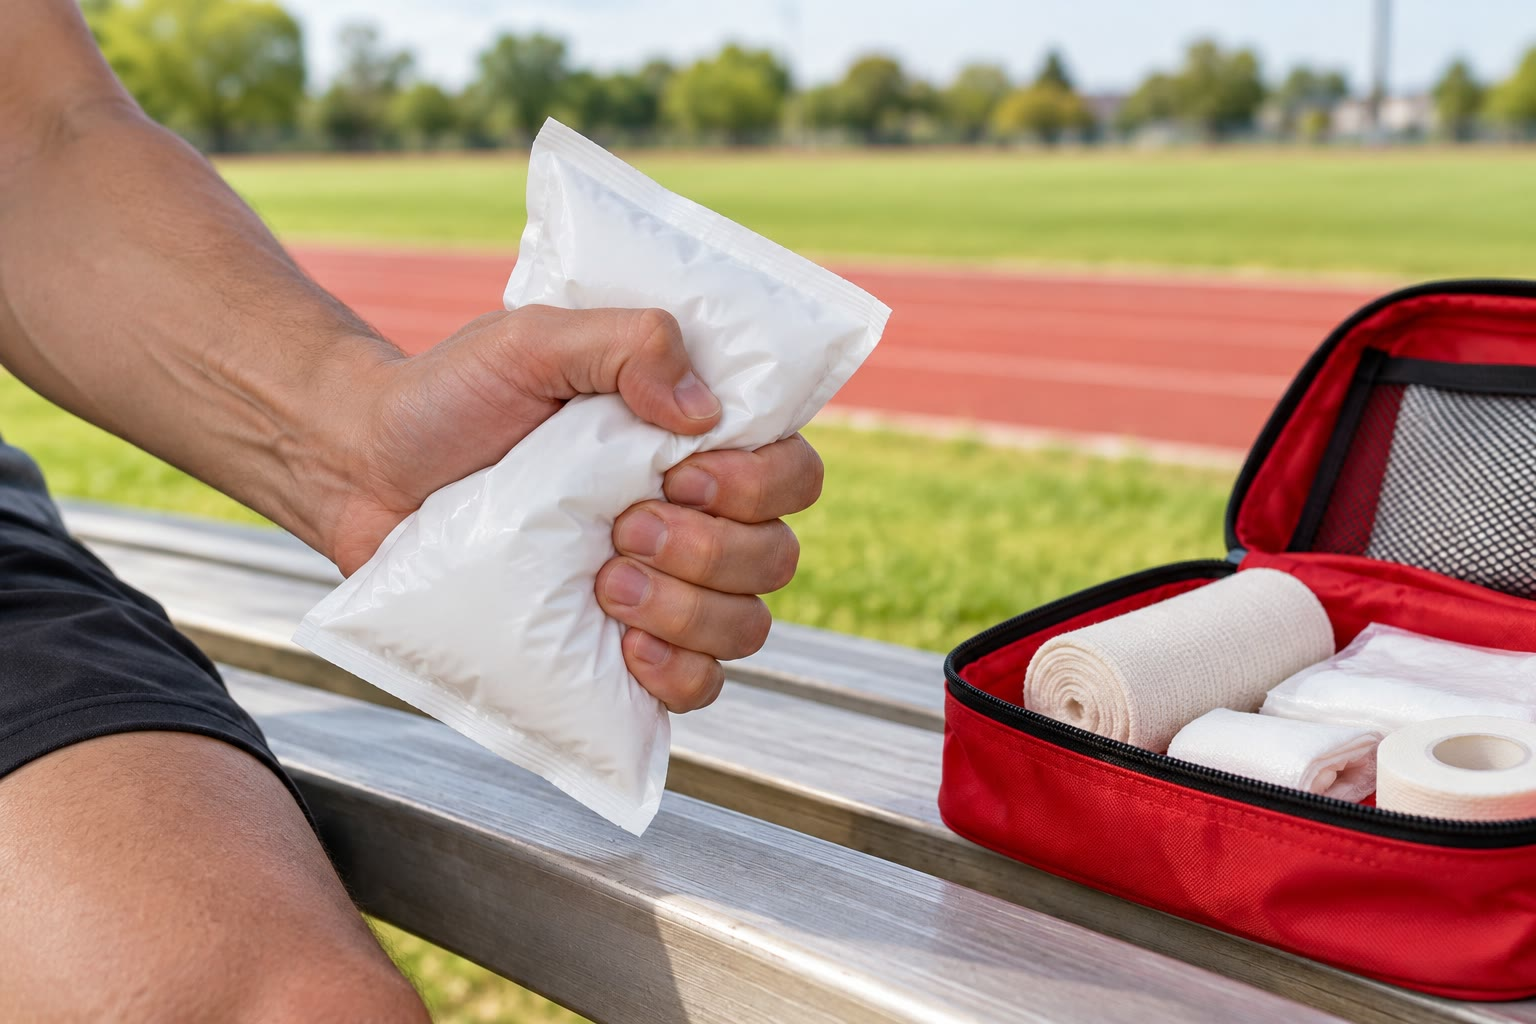
\includegraphics[width=0.55\linewidth]{images/book3/ai/b2-02-cold-pack.jpg}

{\small Een koelpack: wanneer het binnenzakje breekt, lost ammoniumnitraat
op in water en koelt het pack af. Het oplossen is \omterm{def:b2:reaction-enthalpy:exothermic}{endotherm} en
spontaan; de entropie ervan verklaart waarom (\cref{ex:b2:reaction-free-energy:cold-pack}).}
\end{omfigure}

\section{Standaardentropieën en de derde hoofdwet}

Anders dan de enthalpie heeft de entropie een natuurlijk nulpunt.

\begin{theorem}[Derde hoofdwet van de thermodynamica]\label{thm:b2:reaction-free-energy:third-law}
De entropie van een zuiver, volmaakt geordend kristal gaat naar nul wanneer zijn
temperatuur naar \qty{0}{K} gaat.
\end{theorem}
\admitted

\begin{remark}[Waar het nulpunt vandaan komt]\label{rem:b2:reaction-free-energy:third-law}
Walther Nernst stelde in 1906 dat reactie-entropieën tussen gecondenseerde
fasen verdwijnen wanneer $T \to 0$; Max Planck scherpte dat aan tot de bewering
hierboven. De oorsprong is statistisch: entropie telt de microscopische
rangschikkingen die verenigbaar zijn met de toestand van een systeem, en een volmaakt kristal
bij \qty{0}{K} heeft er maar één. Dat tellen gebeurt in het deel van jaar~3,
met toestandssommen.
\end{remark}

\begin{definition}[Molaire standaardentropie]\label{def:b2:reaction-free-energy:standard-entropy}
De \emph{molaire standaardentropie}\index{molaire standaardentropie}
$S^\circ_m(T)$ van een stof is de entropie van één mol ervan in haar
standaardtoestand bij temperatuur $T$, met het nulpunt van de derde hoofdwet.
Anders dan $\Delta_f H^\circ$ is ze een absolute grootheid, positief voor elke
stof, de elementen inbegrepen.
\end{definition}

\begin{proposition}[Absolute entropie uit warmtecapaciteiten]\label{prop:b2:reaction-free-energy:absolute-entropy}
Bij het verwarmen van een stof bij constante druk $p^\circ$ van \qty{0}{K} tot $T$ geldt
\[
  S^\circ_m(T) = \int_0^T\frac{C^\circ_{p,m}(T')}{T'}\,\dd T' +
  \sum_{\text{overgangen}}\frac{\Delta_{\text{trs}}H^\circ}{T_{\text{trs}}} ,
\]
waarbij de integraal in elke fase over haar temperatuurgebied genomen wordt.
\end{proposition}

\begin{proof}
Verwarm de stof reversibel bij constante druk: $\delta S_{\text{c}} =
0$ en $\delta Q = \dd H = C_p\,\dd T$, dus $\dd S = C_p\,\dd T/T$. Bij een
faseovergang (smelten, koken) blijft de temperatuur op $T_{\text{trs}}$
terwijl de warmte $\Delta_{\text{trs}}H$ reversibel wordt opgenomen: de entropie
springt met $\Delta_{\text{trs}}H/T_{\text{trs}}$. Tel de stukken op vanaf het
nulpunt van de derde hoofdwet.
\end{proof}

\begin{omfigure}
\begin{tikzpicture}
\begin{axis}[
  width=0.8\linewidth, height=6.2cm, xmin=0, xmax=1500, ymin=0, ymax=210,
  axis x line=bottom, axis y line=left, xlabel={$T$ (K)},
  ylabel={$S^\circ_m$ van zink (\unit{J/(K.mol)})},
  xtick={0,250,500,750,1000,1250,1500},
  tick label style={font=\small}, label style={font=\small}, clip=false]
\addplot[omDef, very thick, smooth] table[x=T, y=S] {figdata/out/bachelor-2-standard-entropy-solid.dat};
\addplot[omProp, very thick] table[x=T, y=S] {figdata/out/bachelor-2-standard-entropy-liquid.dat};
\addplot[omThm, very thick] table[x=T, y=S] {figdata/out/bachelor-2-standard-entropy-gas.dat};
\draw[densely dashed, gray] (axis cs:692.73,64.6) -- (axis cs:692.73,75.2);
\draw[densely dashed, gray] (axis cs:1180.2,91.9) -- (axis cs:1180.2,189.6);
\node[omDef, font=\small, anchor=south east] at (axis cs:600,60) {vast};
\node[omProp, font=\small, anchor=north west] at (axis cs:850,78) {vloeibaar};
\node[omThm, font=\small, anchor=south] at (axis cs:1350,192) {gas};
\node[font=\scriptsize, anchor=west, align=left] at (axis cs:700,110) {smelten, $+10.6$\\ bij \qty{692.7}{K}};
\node[font=\scriptsize, anchor=east, align=right] at (axis cs:1170,150) {koken,\\ $+97.7$ bij\\ \qty{1180.2}{K}};
\end{axis}
\end{tikzpicture}

{\small \omterm{def:b2:reaction-free-energy:standard-entropy}{Molaire standaardentropie} van zink vanaf het nulpunt van de derde hoofdwet. Ze neemt
toe met de temperatuur naarmate het metaal warmte opslaat, springt dan bij het smeltpunt
met $\Delta_{\text{fus}}H/T_{\text{fus}}$ en, veel meer, bij het kookpunt
met $\Delta_{\text{vap}}H/T_b$: een gas is veel wanordelijker dan een
vloeistof.}
% ledger: s0T:Zn_crl.0, s0T:Zn_crl.298.15, s0T:Zn_cr.692, s0T:Zn_l.692, s0T:Zn_l.1180, s0T:Zn_g.1180, hT:Zn_cr.692, hT:Zn_l.692, hT:Zn_l.1180, hT:Zn_g.1180, dfh:Zn_g (curve in figdata/bachelor-2/standard-entropy.py)
\end{omfigure}

De figuur geeft ordes van grootte die het onthouden waard zijn. Bij
kamertemperatuur heeft een metaal of een hard kristal enkele tientallen
\unit{J/(K.mol)}, een vloeistof rond de honderd, een gas honderd tot driehonderd;
smelten voegt een beetje toe, koken veel. De molaire standaardentropieën
die in dit deel gebruikt worden, staan in de tabellen naast de vormingsenthalpieën.

\section{Reactie-entropie}

\begin{definition}[Reactie-entropie]\label{def:b2:reaction-free-energy:reaction-entropy}
De \emph{reactie-entropie}\index{reactie-entropie} is $\Delta_r S =
(\partial S/\partial\xi)_{T,p}$, en de
\emph{standaardreactie-entropie}\index{standaardreactie-entropie} is $\Delta_r S^\circ(T) =
\sum_i\nu_iS^\circ_{m,i}(T)$, in \unit{J/(K.mol)}.
\end{definition}

Omdat standaardentropieën absoluut zijn, is er geen vormingsreactie nodig:
de elementen tellen mee met hun eigen entropie.

\begin{example}[Drie reactie-entropieën]\label{ex:b2:reaction-free-energy:entropies}
Bij \qty{298.15}{K}:
\begin{itemize}
  \item \ce{CaCO3(s) -> CaO(s) + CO2(g)}: $\Delta_r S^\circ = 39.75 + 213.79 -
        92.9 = \qty{+160.6}{J/(K.mol)}$, een gas dat uit een vaste stof ontstaat;
  \item \ce{N2(g) + 3H2(g) -> 2NH3(g)}: $\Delta_r S^\circ = 2(192.77) -
        191.61 - 3(130.68) = \qty{-198.1}{J/(K.mol)}$, vier gasmoleculen
        die er twee worden;
  \item \ce{N2O4(g) -> 2NO2(g)}: $\Delta_r S^\circ = 2(240.03) - 304.38 =
        \qty{+175.7}{J/(K.mol)}$.
\end{itemize}
% ledger: s0:CaCO3_cr, s0:CaO_cr, s0:CO2_g, s0:N2_g, s0:H2_g, s0:NH3_g, s0:N2O4_g, s0:NO2_g (computed in figdata/bachelor-2/thermo-data.py)
\end{example}

\begin{proposition}[Het teken van een reactie-entropie]\label{prop:b2:reaction-free-energy:sign-rule}
Wanneer gassen deelnemen, is het teken van $\Delta_r S^\circ$ in het algemeen dat van
$\Delta\nu_{\text{gas}} = \sum_{\text{gassen}}\nu_i$, en de grootte ongeveer
\qty{100}{} tot \qty{200}{J/(K.mol)} per mol gevormd of verbruikt gas. Wanneer
$\Delta\nu_{\text{gas}} = 0$, of er geen gas meedoet, is $\Delta_r S^\circ$
klein en moet het teken berekend worden.
\end{proposition}

\begin{proof}[Verantwoording]
De molaire entropie van een gas bij \qty{298}{K} ligt tussen 130 en
\qty{300}{J/(K.mol)}, die van een vaste stof of een vloeistof bij enkele tientallen: het vormen of
verbruiken van één mol gas overheerst elke andere bijdrage. Dit is een
vuistregel, geen stelling: het oplossen van een zout, zonder gas, kan
de entropie toch met honderd \unit{J/(K.mol)} veranderen.
\end{proof}

\begin{method}[Het teken van $\Delta_r S^\circ$ voorspellen]\label{met:b2:reaction-free-energy:entropy-sign}
\begin{enumerate}
  \item Tel $\Delta\nu_{\text{gas}}$: als die niet nul is, geeft ze het
        teken.
  \item Vergelijk anders de orde van de toestanden: een kristal oplossen,
        smelten, een molecuul in twee stukken breken verhogen de entropie;
        neerslaan, bevriezen, twee moleculen tot één verbinden verlagen haar.
  \item Wanneer de beslissing ertoe doet, bereken $\sum_i\nu_iS^\circ_{m,i}$.
\end{enumerate}
\end{method}

Het deel van jaar~1 kwam een gevolg tegen: een eliminatie maakt meer moleculen
dan een substitutie met dezelfde reagentia (het alkeen, de vertrekkende groep
en de geprotoneerde base, tegenover het substitutieproduct en de vertrekkende
groep). Haar \omterm{def:b2:reaction-free-energy:reaction-entropy}{reactie-entropie} is groter, en de entropieterm, die met de temperatuur
toeneemt zoals de volgende paragraaf laat zien, verklaart waarom warmte
eliminatie boven substitutie bevoordeelt.

\section{De gibbsenergie}

\begin{definition}[Gibbsenergie]\label{def:b2:reaction-free-energy:gibbs-energy}
De \emph{gibbsenergie}\index{gibbsenergie} (of vrije enthalpie) van een systeem
is de toestandsfunctie $G = H - TS$, extensief, in joule.
\end{definition}

\begin{definition}[Reactie-gibbsenergie]\label{def:b2:reaction-free-energy:reaction-gibbs}
De \emph{reactie-gibbsenergie}\index{reactie-gibbsenergie} is $\Delta_r G
= (\partial G/\partial\xi)_{T,p}$, en de
\emph{standaardreactie-gibbsenergie}\index{standaardreactie-gibbsenergie} is $\Delta_r G^\circ(T) =
\sum_i\nu_iG^\circ_{m,i}(T)$, beide in \unit{kJ/mol}.
\end{definition}

\begin{proposition}[Enthalpie- en entropieterm]\label{prop:b2:reaction-free-energy:g-h-s}
$\Delta_r G = \Delta_r H - T\Delta_r S$, en $\Delta_r G^\circ = \Delta_r
H^\circ - T\Delta_r S^\circ$.
\end{proposition}

\begin{proof}
Differentieer $G = H - TS$ naar $\xi$ bij vaste $T$ en $p$: $T$
is een constante voor de afgeleide.
\end{proof}

\begin{proposition}[Differentiaal van $G$ voor een reagerend systeem]\label{prop:b2:reaction-free-energy:dG}
Voor een gesloten systeem waarin één reactie plaatsvindt, bij uniforme $T$ en
$p$, geldt
\[
  \dd G = V\,\dd p - S\,\dd T + \Delta_r G\,\dd\xi .
\]
\end{proposition}

\begin{proof}
$G(T, p, \xi)$ heeft de totale differentiaal $\dd G = (\partial G/\partial
T)_{p,\xi}\dd T + (\partial G/\partial p)_{T,\xi}\dd p + \Delta_r G\,\dd\xi$.
De eerste twee partiële afgeleiden worden bij vaste samenstelling genomen: het zijn
die van een gesloten systeem met vaste samenstelling, waarvoor de natuurkunde
$\dd U = T\dd S - p\dd V$ geeft, zodat $\dd G = \dd U + p\dd V + V\dd p - T\dd S
- S\dd T = V\dd p - S\dd T$. Dus $(\partial G/\partial T)_{p,\xi} = -S$
en $(\partial G/\partial p)_{T,\xi} = V$.
\end{proof}

\section{Het evolutiecriterium}

\begin{theorem}[Evolutiecriterium]\label{thm:b2:reaction-free-energy:evolution}
In een gesloten systeem dat op constante temperatuur en druk gehouden wordt en geen
andere arbeid uitwisselt dan die van de drukkrachten, kan een reactie alleen voortschrijden in
de richting waarvoor
\[
  \Delta_r G\,\dd\xi \leq 0 ,
\]
met gelijkheid bij evenwicht. Als $\Delta_r G < 0$ verloopt de reactie
voorwaarts, als $\Delta_r G > 0$ achterwaarts, en het systeem is in
evenwicht wanneer $\Delta_r G = 0$.
\end{theorem}

\begin{proof}
Neem een oneindig kleine verandering bij uniforme $T$ en $p$, gelijk aan die van de
omgeving. De eerste hoofdwet met alleen volumearbeid geeft $\dd U = \delta Q
- p\dd V$; de tweede geeft $\delta Q = T\dd S - T\delta S_{\text{c}}$. Dan is
\[
  \dd G = \dd U + p\dd V + V\dd p - T\dd S - S\dd T = -T\,\delta
  S_{\text{c}} + V\dd p - S\dd T .
\]
Vergelijken met \cref{prop:b2:reaction-free-energy:dG} geeft bij vaste $T$ en $p$:
$\Delta_r G\,\dd\xi = -T\,\delta S_{\text{c}}$. Omdat $\delta S_{\text{c}}
\geq 0$, is $\Delta_r G\,\dd\xi \leq 0$, en $\delta S_{\text{c}} = 0$ (een
reversibele verandering, in evenwicht) vereist $\Delta_r G = 0$.
\end{proof}

\begin{remark}[Wat het criterium zegt, en wat niet]\label{rem:b2:reaction-free-energy:criterion}
De entropie die een reactie bij constante $T$ en $p$ creëert, is $-\Delta_r G\,
\dd\xi/T$: de \omterm{def:b2:reaction-free-energy:gibbs-energy}{gibbsenergie} is de tweede hoofdwet, beperkt tot de omstandigheden
van het laboratorium en geschreven met grootheden van het systeem alleen. Ze zegt
in welke richting een reactie mag verlopen, nooit hoe snel: diamant, waarvoor
de omzetting in grafiet $\Delta_r G^\circ < 0$ heeft, blijft eeuwig bestaan in een
ring. En ze veronderstelt dat er geen andere arbeid is: een cel die elektrische arbeid levert, of een
elektrolysecel die er ontvangt, gehoorzaamt aan een aangepast criterium
(\cref{ch:b2:cell-thermodynamics}).
\end{remark}

\begin{definition}[Exergonisch en endergonisch]\label{def:b2:reaction-free-energy:exergonic}
Een reactie is \emph{exergonisch}\index{exergonisch} in een gegeven toestand wanneer
$\Delta_r G < 0$ en \emph{endergonisch}\index{endergonisch} wanneer $\Delta_r G >
0$. Met elk deeltje in zijn standaardtoestand slaan deze woorden op het teken
van $\Delta_r G^\circ$.
\end{definition}

Het criterium gebruikt $\Delta_r G$, de waarde in de werkelijke toestand van het
systeem; $\Delta_r G^\circ$ verwijst naar elk deeltje in zijn standaardtoestand,
wat zelden de toestand van een echt mengsel is. Het verband tussen beide, via
de samenstelling, is het onderwerp van \cref{ch:b2:chemical-potential}, en
levert de wet $Q = K^\circ$ van jaar~1 in \cref{ch:b2:equilibrium-shifts}. Voor
reacties tussen zuivere vaste stoffen en vloeistoffen, en gassen bij \qty{1}{bar}, vallen
beide samen.

\begin{example}[Het koelpack]\label{ex:b2:reaction-free-energy:cold-pack}
Voor \ce{NH4NO3(s) -> NH4+(aq) + NO3-(aq)} bij \qty{298.15}{K}, in de
standaardtoestand: $\Delta_r H^\circ = -339.87 + 365.56 = \qty{+25.69}{kJ/mol}$ en
$\Delta_r S^\circ = 259.8 - 151.08 = \qty{+108.7}{J/(K.mol)}$, dus
$\Delta_r G^\circ = 25.69 - 298.15 \times 0.1087 = \qty{-6.7}{kJ/mol}$: het
oplossen is \omterm{def:b2:reaction-enthalpy:exothermic}{endotherm} en \omterm{def:b2:reaction-free-energy:exergonic}{exergonisch}. De ionen, vrij in het water, zijn
wanordelijker dan in het kristal, en de entropieterm $T\Delta_r
S^\circ = \qty{32.4}{kJ/mol}$ weegt zwaarder dan de kosten aan enthalpie.
% ledger: dfh:NH4NO3_cr, s0:NH4NO3_cr, dfh:NH4NO3_ai, s0:NH4NO3_ai (computed in figdata/bachelor-2/thermo-data.py)
\end{example}

\begin{history}[Josiah Willard Gibbs]
\begin{minipage}[t]{0.2\linewidth}\vspace{0pt}
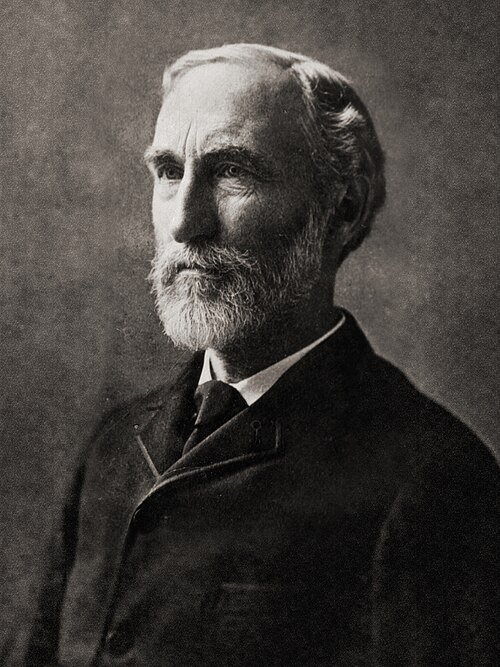
\includegraphics[width=\linewidth]{images/book3/gibbs.jpg}
\end{minipage}\hfill
\begin{minipage}[t]{0.76\linewidth}\vspace{0pt}
Josiah Willard Gibbs (1839--1903), hoogleraar mathematische fysica aan
Yale, publiceerde tussen 1876 en 1878 \emph{On the Equilibrium of
Heterogeneous Substances}, zo'n driehonderd bladzijden in de verhandelingen van
een kleine academie, waarin de vrije energie, de chemische potentiaal en de
faseregel van de volgende hoofdstukken allemaal voorkomen. Weinig chemici lazen het tot het
in de jaren 1890 vertaald werd. (Foto: publiek domein, Wikimedia
Commons.)
\end{minipage}
\end{history}

\section{Standaardreactie-gibbsenergieën en temperatuur}

\begin{definition}[Benadering van Ellingham]\label{def:b2:reaction-free-energy:ellingham-approximation}
De \emph{benadering van Ellingham}\index{benadering van Ellingham} beschouwt
$\Delta_r H^\circ$ en $\Delta_r S^\circ$ als onafhankelijk van de temperatuur
over een interval zonder faseovergang. Dan is $\Delta_r G^\circ(T)
= \Delta_r H^\circ - T\Delta_r S^\circ$ een rechte in $T$, met helling
$-\Delta_r S^\circ$.
\end{definition}

\begin{proposition}[Afgeleiden naar de temperatuur]\label{prop:b2:reaction-free-energy:gibbs-helmholtz}
\[
  \frac{\dd\Delta_r G^\circ}{\dd T} = -\Delta_r S^\circ, \qquad
  \frac{\dd}{\dd T}\!\left(\frac{\Delta_r G^\circ}{T}\right) =
  -\frac{\Delta_r H^\circ}{T^2}\ \ \text{(Gibbs--Helmholtz)}, \qquad
  \frac{\dd\Delta_r S^\circ}{\dd T} = \frac{\Delta_r C^\circ_p}{T}.
\]
In het bijzonder geldt de \omterm{def:b2:reaction-free-energy:ellingham-approximation}{benadering van Ellingham} wanneer $\Delta_r C^\circ_p$
klein is.
\end{proposition}

\begin{proof}
Met elk deeltje in zijn standaardtoestand heeft $G^\circ(T, \xi)$ als afgeleide $(\partial
G^\circ/\partial T)_\xi = -S^\circ$ (\cref{prop:b2:reaction-free-energy:dG}).
Volgens de stelling van Schwarz is
\[
  \frac{\dd\Delta_r G^\circ}{\dd T} = \partial_\xi\partial_T G^\circ =
  -\partial_\xi S^\circ = -\Delta_r S^\circ .
\] Verder is $\frac{\dd}{\dd
T}(\Delta_r G^\circ/T) = \frac{-T\Delta_r S^\circ - \Delta_r G^\circ}{T^2} =
-\frac{\Delta_r H^\circ}{T^2}$. Ten slotte is $\dd S^\circ_m = C^\circ_{p,m}\,\dd
T/T$ voor elk deeltje (\cref{prop:b2:reaction-free-energy:absolute-entropy}),
en dezelfde combinatie geeft de laatste betrekking. Als $\Delta_r C^\circ_p$
klein is, veranderen $\Delta_r H^\circ$ (Kirchhoff) en $\Delta_r S^\circ$ nauwelijks.
\end{proof}

\begin{definition}[Inversietemperatuur]\label{def:b2:reaction-free-energy:inversion-temperature}
Wanneer $\Delta_r H^\circ$ en $\Delta_r S^\circ$ hetzelfde teken hebben, is de
\emph{inversietemperatuur}\index{inversietemperatuur} van de reactie
de temperatuur waarbij $\Delta_r G^\circ$ van teken verandert; in de \omterm{def:b2:reaction-free-energy:ellingham-approximation}{benadering van
Ellingham} is $T_i = \Delta_r H^\circ/\Delta_r S^\circ$.
\end{definition}

\begin{omfigure}
\begin{tikzpicture}
\begin{axis}[
  width=0.72\linewidth, height=5.6cm, xmin=0, xmax=1600, ymin=0, ymax=260,
  axis x line=bottom, axis y line=left, xlabel={$T$ (K)}, ylabel={\unit{kJ/mol}},
  tick label style={font=\small}, label style={font=\small}, clip=false]
\addplot[omThm, very thick] table[x=T, y=DrH] {figdata/out/bachelor-2-thermo-data-calcite.dat};
\addplot[omDef, very thick] table[x=T, y=TDrS] {figdata/out/bachelor-2-thermo-data-calcite.dat};
\node[omThm, anchor=south west, font=\small] at (axis cs:60,180) {$\Delta_r H^\circ = 178.3$};
\node[omDef, anchor=west, font=\small] at (axis cs:1600,257) {$T\Delta_r S^\circ$};
\draw[dotted] (axis cs:1110,0) -- (axis cs:1110,178.3);
\node[anchor=south west, font=\small] at (axis cs:1120,8) {$T_i = \qty{1110}{K}$};
\node[font=\scriptsize, align=center] at (axis cs:600,140) {$\Delta_r G^\circ > 0$:\\ calciet stabiel};
\node[font=\scriptsize, align=center] at (axis cs:1470,206) {$\Delta_r G^\circ < 0$};
\end{axis}
\end{tikzpicture}

{\small De enthalpie- en entropieterm van \ce{CaCO3(s) -> CaO(s) + CO2(g)}
in de \omterm{def:b2:reaction-free-energy:ellingham-approximation}{benadering van Ellingham}. Onder de \omterm{def:b2:reaction-free-energy:inversion-temperature}{inversietemperatuur} wint de
enthalpiekost en is kalksteen stabiel onder \qty{1}{bar}
koolstofdioxide; erboven wint de entropieterm en ontleedt kalksteen.}
% ledger: dfh:CaCO3_cr, dfh:CaO_cr, dfh:CO2, s0:CaCO3_cr, s0:CaO_cr, s0:CO2_g (computed in figdata/bachelor-2/thermo-data.py)
\end{omfigure}

\begin{omfigure}
\begin{tikzpicture}[font=\small]
  \draw[thick] (0,0) rectangle (8,4);
  \draw[thick] (4,0) -- (4,4) (0,2) -- (8,2);
  \node[above] at (2,4) {$\Delta_r H^\circ < 0$};
  \node[above] at (6,4) {$\Delta_r H^\circ > 0$};
  \node[left] at (0,3) {$\Delta_r S^\circ > 0$};
  \node[left] at (0,1) {$\Delta_r S^\circ < 0$};
  \node[align=center, omDef] at (2,3) {exergonisch\\ bij elke $T$};
  \node[align=center, omProp] at (6,3) {exergonisch\\ boven $T_i$};
  \node[align=center, omProp] at (2,1) {exergonisch\\ onder $T_i$};
  \node[align=center, omThm] at (6,1) {endergonisch\\ bij elke $T$};
\end{tikzpicture}

{\small De vier gevallen van $\Delta_r G^\circ = \Delta_r H^\circ - T\Delta_r
S^\circ$ (\omterm{def:b2:reaction-free-energy:ellingham-approximation}{benadering van Ellingham}). Verbrandingen staan in het vak linksboven;
de ontleding van kalksteen en het koelpack rechtsboven; de
ammoniaksynthese linksonder.}
\end{omfigure}

\begin{method}[Een standaardreactie-gibbsenergie bij temperatuur $T$]\label{met:b2:reaction-free-energy:delta-g-standard}
\begin{enumerate}
  \item Bereken uit de tabellen bij \qty{298.15}{K} $\Delta_r H^\circ$ en
        $\Delta_r S^\circ$.
  \item Controleer dat geen enkel deeltje van toestand verandert tussen \qty{298}{K} en $T$;
        tel anders de overgang (enthalpie en entropie) erbij of vertrek vanuit
        de nieuwe toestand.
  \item In de \omterm{def:b2:reaction-free-energy:ellingham-approximation}{benadering van Ellingham} is $\Delta_r G^\circ(T) = \Delta_r H^\circ
        - T\Delta_r S^\circ$.
  \item Waar $\Delta_r C^\circ_p$ niet klein is of het interval lang,
        gebruik je rechtstreeks getabelleerde $\Delta_f G^\circ(T)$.
\end{enumerate}
\end{method}

\begin{example}[Twee toetsen van de benadering]\label{ex:b2:reaction-free-energy:tests}
Voor kalksteen is $\Delta_r C^\circ_p = 42.80 + 37.13 - 81.88 =
\qty{-2.0}{J/(K.mol)}$: de benadering is uitstekend, en $\Delta_r
G^\circ = 178.3 - T \times 0.1606$ geeft $T_i = \qty{1110}{K}$. Voor ammoniak
is $\Delta_r G^\circ(700) \approx -91.9 + 700 \times 0.1981 =
\qty{+46.8}{kJ/mol}$, terwijl de tabellen $2\Delta_f G^\circ(\ce{NH3}, 700) =
\qty{+54.4}{kJ/mol}$ geven: hier is $\Delta_r C^\circ_p = \qty{-44}{J/(K.mol)}$ en
de fout bedraagt \qty{8}{kJ/mol}, een factor 4 op de evenwichtsconstante bij
die temperatuur.
% ledger: cp:CaO_cr.298, cp:CO2_g.298, cp:CaCO3_cr.298, janafG:NH3.700 (computed in figdata/bachelor-2/thermo-data.py)
\end{example}

\section{Oefeningen}

\begin{exercise}[$\star$]\label{exo:b2:reaction-free-energy:1}
Voorspel het teken van $\Delta_r S^\circ$ voor: (a) \ce{2H2(g) + O2(g) -> 2H2O(l)};
(b) \ce{CaCO3(s) -> CaO(s) + CO2(g)}; (c) \ce{N2O4(g) -> 2NO2(g)};
(d) \ce{Ag+(aq) + Cl-(aq) -> AgCl(s)}; (e) \ce{H2O(s) -> H2O(l)};
(f) \ce{H2(g) + Cl2(g) -> 2HCl(g)}.
\end{exercise}

\begin{exercise}[$\star$]\label{exo:b2:reaction-free-energy:2}
Bereken $\Delta_r S^\circ$ en $\Delta_r G^\circ$ bij \qty{298.15}{K} voor de
ammoniaksynthese, \ce{N2(g) + 3H2(g) -> 2NH3(g)}, met $\Delta_r
H^\circ = \qty{-91.9}{kJ/mol}$ en de entropieën van het hoofdstuk. Is ze
\omterm{def:b2:reaction-free-energy:exergonic}{exergonisch}?
\end{exercise}

\begin{exercise}[$\star$]\label{exo:b2:reaction-free-energy:3}
Bereken $\Delta_r G^\circ(\qty{298.15}{K})$ van \ce{H2(g) + 1/2O2(g) ->
H2O(l)} uit $\Delta_f H^\circ(\ce{H2O}, \text{l}) = \qty{-285.83}{kJ/mol}$
en de standaardentropieën \ce{H2(g)} 130.68, \ce{O2(g)} 205.15,
\ce{H2O(l)} \qty{69.95}{J/(K.mol)}. Waarom is deze waarde de
standaardvormingsgibbsenergie van vloeibaar water?
% ledger: dfh:H2O-l, s0:H2_g, s0:O2_g, s0:H2O_l
\end{exercise}

\begin{exercise}[$\star$]\label{exo:b2:reaction-free-energy:4}
Lees op de figuur van de entropie van zink de \omterm{def:b2:reaction-free-energy:standard-entropy}{molaire standaardentropie} af bij
\qty{298}{K} en bij \qty{1000}{K}, en de sprongen bij het smelt- en het
kookpunt. Leid daaruit de smelt- en de verdampingsenthalpie af.
\end{exercise}

\begin{exercise}[$\star\star$]\label{exo:b2:reaction-free-energy:5}
Bereken voor \ce{H2O(l) -> H2O(g)} bij \qty{298.15}{K} $\Delta_r H^\circ$,
$\Delta_r S^\circ$ en $\Delta_r G^\circ$ uit de tabellen van het hoofdstuk.
Leg uit waarom $\Delta_r S^\circ \neq \Delta_r H^\circ/T$ bij \qty{298}{K} en wat
de positieve $\Delta_r G^\circ$ betekent, en schat in de \omterm{def:b2:reaction-free-energy:ellingham-approximation}{benadering van
Ellingham} de temperatuur waarbij vloeibaar water en zijn damp bij
\qty{1}{bar} in evenwicht zijn. Vergelijk met het kookpunt.
\end{exercise}

\begin{exercise}[$\star\star$]\label{exo:b2:reaction-free-energy:6}
Voor \ce{N2O4(g) -> 2NO2(g)} is $\Delta_r H^\circ = \qty{57.1}{kJ/mol}$ en
$\Delta_r S^\circ = \qty{175.7}{J/(K.mol)}$. Bereken de
\omterm{def:b2:reaction-free-energy:inversion-temperature}{inversietemperatuur}, en leg uit waarom een dichtgesmolten buis met het bruine gas \ce{NO2} bleker wordt
wanneer ze in ijs wordt afgekoeld.
\end{exercise}

\begin{exercise}[$\star\star$]\label{exo:b2:reaction-free-energy:7}
Een reactie heeft $\Delta_r G^\circ = \qty{-12.0}{kJ/mol}$ bij \qty{300}{K}
en $\qty{-4.0}{kJ/mol}$ bij \qty{400}{K}. Bepaal in de \omterm{def:b2:reaction-free-energy:ellingham-approximation}{benadering van Ellingham}
$\Delta_r H^\circ$ en $\Delta_r S^\circ$, en controleer de
betrekking van Gibbs--Helmholtz.
\end{exercise}

\begin{exercise}[$\star\star$]\label{exo:b2:reaction-free-energy:8}
Bereken $\Delta_r G^\circ$ van de vorming van methaan, \ce{C(s) + 2H2(g) ->
CH4(g)}, bij \qty{298.15}{K}, uit $\Delta_f H^\circ = \qty{-74.87}{kJ/mol}$
en de entropieën \ce{C} (grafiet) 5.74, \ce{H2} 130.68, \ce{CH4}
\qty{186.25}{J/(K.mol)}. Boven welke temperatuur wordt methaan
instabiel ten opzichte van zijn elementen onder de standaarddruk?
% ledger: dfh:CH4_g, s0:C_gr, s0:H2_g, s0:CH4_g
\end{exercise}

\begin{exercise}[$\star\star$]\label{exo:b2:reaction-free-energy:9}
Een halogeenalkaan reageert met een base door substitutie of door eliminatie. Schrijf
beide reacties op voor 2-broompropaan en hydroxide. Bepaal met $\Delta_r
H^\circ(\text{eliminatie}) - \Delta_r H^\circ(\text{substitutie}) =
\qty{+40}{kJ/mol}$ en $\Delta_r S^\circ(\text{eliminatie}) - \Delta_r
S^\circ(\text{substitutie}) = \qty{+90}{J/(K.mol)}$ (ordes van grootte)
boven welke temperatuur de eliminatie de meest exergonische van
de twee wordt, en leg de rol van het aantal moleculen uit.
\end{exercise}

\begin{exercise}[$\star\star\star$]\label{exo:b2:reaction-free-energy:10}
Kristallijn koolstofmonoxide bereikt bij \qty{0}{K} geen entropie nul: elk
molecuul kan als CO of als OC zitten, bijna willekeurig, omdat de twee oriëntaties
vrijwel dezelfde energie hebben. Bereken, met de formule van Boltzmann $S = k_B\ln W$, waarin
$W$ het aantal rangschikkingen is (geteld in het deel van jaar~3), de
residuele molaire entropie. Waarom geldt de derde hoofdwet niet voor dit
kristal?
\end{exercise}

\begin{exercise}[$\star\star\star$]\label{exo:b2:reaction-free-energy:11}
Toon aan dat als $\Delta_r C^\circ_p$ een constante $c$ is,
$\Delta_r S^\circ(T) = \Delta_r S^\circ(T_0) + c\ln(T/T_0)$ en
$\Delta_r G^\circ(T) = \Delta_r H^\circ(T_0) - T\Delta_r S^\circ(T_0) +
c\,[T - T_0 - T\ln(T/T_0)]$. Pas dit toe op kalksteen ($c =
\qty{-2.0}{J/(K.mol)}$) bij \qty{1100}{K}, en meet de fout van de
\omterm{def:b2:reaction-free-energy:ellingham-approximation}{benadering van Ellingham}.
\end{exercise}

\begin{exercise}[$\star\star\star$]\label{exo:b2:reaction-free-energy:12}
Titaan wordt gemaakt uit zijn oxide, rutiel, via zijn chloride. (a) Bereken
$\Delta_r H^\circ$ en $\Delta_r S^\circ$ bij \qty{298}{K} van \ce{TiO2(s) +
2Cl2(g) -> TiCl4(g) + O2(g)}, met \ce{TiO2} ($-944.0$ \unit{kJ/mol},
\qty{50.62}{J/(K.mol)}) en \ce{TiCl4(g)} ($-763.2$, 353.2), en de
$\Delta_r G^\circ$ ervan bij \qty{1000}{K} in de \omterm{def:b2:reaction-free-energy:ellingham-approximation}{benadering van Ellingham}.
(b) Er wordt koolstof toegevoegd: \ce{C(s) + O2(g) -> CO2(g)}, $\Delta_r H^\circ =
\qty{-393.5}{kJ/mol}$, $\Delta_r S^\circ = \qty{+2.9}{J/(K.mol)}$. Bereken
$\Delta_r G^\circ(\qty{1000}{K})$ van de som van de twee reacties en
leg uit hoe de tweede de eerste aandrijft.
% ledger: dfh:TiO2_cr, s0:TiO2_cr, dfh:TiCl4_g, s0:TiCl4_g, s0:Cl2_g, s0:O2_g, s0:C_gr, s0:CO2_g
\end{exercise}

\section{Probleem: de kalkoven}

\begin{problem}[{Weekendprobleem --- de entropie en de enthalpie van een
ontleding, haar gibbsenergie als functie van de temperatuur, het evolutiecriterium
in een oven, en de energie en het koolstofdioxide van een ton
ongebluste kalk}]
\label{pb:b2:reaction-free-energy:1}
Ongebluste kalk, \ce{CaO}, wordt gemaakt door kalksteen, \ce{CaCO3}, in een oven te verhitten. Gegevens bij
\qty{298.15}{K}: $\Delta_f H^\circ$ (\unit{kJ/mol}) \ce{CaCO3(s)}
$-1206.92$, \ce{CaO(s)} $-635.09$, \ce{CO2(g)} $-393.51$; $S^\circ_m$
(\unit{J/(K.mol)}) 92.9, 39.75, 213.79; $C^\circ_{p,m}$ (\unit{J/(K.mol)})
81.88, 42.80, 37.13. Molaire massa's: \ce{CaO} \qty{56.08}{g/mol}, \ce{CO2}
\qty{44.01}{g/mol}, \ce{CH4} \qty{16.04}{g/mol}; verbranding van methaan,
water als damp, $\Delta_r H^\circ = \qty{-802.3}{kJ/mol}$.
% ledger: dfh:CaCO3_cr, dfh:CaO_cr, dfh:CO2, s0:CaCO3_cr, s0:CaO_cr, s0:CO2_g, cp:CaCO3_cr.298, cp:CaO_cr.298, cp:CO2_g.298

\medskip
\noindent\textbf{Deel I --- Bij kamertemperatuur.}
\begin{enumerate}
  \item Schrijf de ontleding van kalksteen op.
  \item Bereken $\Delta_r H^\circ(\qty{298}{K})$. Is de reactie \omterm{def:b2:reaction-enthalpy:exothermic}{exotherm}?
  \item Bereken $\Delta_r S^\circ(\qty{298}{K})$ en verklaar het teken.
  \item Bereken $\Delta_r G^\circ(\qty{298}{K})$.
  \item Is kalksteen bij kamertemperatuur stabiel onder \qty{1}{bar}
        koolstofdioxide? Waarom blijven kalksteenkliffen bestaan?
  \item Bereken $\Delta_r C^\circ_p$, en zeg wat het betekent voor de
        temperatuurafhankelijkheid van $\Delta_r H^\circ$ en $\Delta_r S^\circ$.
\end{enumerate}

\medskip
\noindent\textbf{Deel II --- Verhitten.}
\begin{enumerate}[resume]
  \item Schrijf $\Delta_r G^\circ(T)$ op in de \omterm{def:b2:reaction-free-energy:ellingham-approximation}{benadering van Ellingham}.
  \item Bereken het bij \qty{1000}{K} en bij \qty{1300}{K}.
  \item Bereken de \omterm{def:b2:reaction-free-energy:inversion-temperature}{inversietemperatuur} $T_i$.
  \item Controleer de betrekking van Gibbs--Helmholtz op deze uitdrukking.
  \item Schat met de formule van \cref{exo:b2:reaction-free-energy:11}
        de verandering van $\Delta_r G^\circ$ bij $T_i$ die
        $\Delta_r C^\circ_p$ veroorzaakt, en de verschuiving van $T_i$ die daaruit volgt.
\end{enumerate}

\medskip
\noindent\textbf{Deel III --- De oven.}
In dit deel staat het koolstofdioxide boven de vaste stoffen op \qty{1}{bar}, zodat
$\Delta_r G = \Delta_r G^\circ$.
\begin{enumerate}[resume]
  \item Wat zegt het evolutiecriterium bij \qty{1000}{K}? En bij
        \qty{1300}{K}?
  \item Wat gebeurt er met een mengsel van ongebluste kalk en koolstofdioxide bij
        \qty{1}{bar} dat afgekoeld wordt tot onder $T_i$?
  \item Hoeveel entropie wordt er gecreëerd per mol kalksteen die bij
        \qty{1300}{K} ontleedt?
  \item Ovens worden doorstroomd door de verbrandingsgassen, die armer zijn aan koolstofdioxide.
        Raad, vóór het volgende hoofdstuk, of dat de
        ontleding helpt.
\end{enumerate}

\medskip
\noindent\textbf{Deel IV --- Een ton ongebluste kalk.}
\begin{enumerate}[resume]
  \item Bereken de hoeveelheid ongebluste kalk in één ton.
  \item Bereken de warmte die de reactie opneemt per ton ongebluste kalk
        (neem $\Delta_r H^\circ$ constant).
  \item Bereken de massa koolstofdioxide die de kalksteen vrijgeeft per
        ton ongebluste kalk.
  \item De warmte komt van het verbranden van methaan met een nuttig rendement van
        50\,\%. Bereken de massa methaan die per ton ongebluste kalk verbrand wordt.
  \item Bereken het koolstofdioxide dat uit dit methaan komt.
  \item Bereken het totale koolstofdioxide per ton ongebluste kalk, en het aandeel
        dat van de kalksteen zelf komt.
  \item Waarom kan een schonere brandstof slechts een deel van deze uitstoot verminderen?
  \item Geef de temperatuur waarboven kalksteen ontleedt onder
        \qty{1}{bar} koolstofdioxide.
\end{enumerate}
\end{problem}
